\documentclass{amsart}
\usepackage[utf8]{inputenc}
\usepackage{tikz}
\usetikzlibrary{decorations.pathreplacing}
\usetikzlibrary{shapes.multipart}
\usepackage{forest}
\usepackage{algorithm}
\usepackage{algpseudocode}
\usepackage{wrapfig}
\usepackage{amsmath}
\usepackage{stix2}
\usepackage{mdframed}
% Defining mdframed definition
\mdfdefinestyle{Example}{%
	linecolor=black,
	innertopmargin=\baselineskip,
	innerbottommargin=\baselineskip,
	innerrightmargin=20pt,
	innerleftmargin=20pt,
	skipabove=5pt,
	skipbelow=5pt,
	backgroundcolor=green!5}

\mdfdefinestyle{Quiz}{%
	linecolor=black,
	innertopmargin=\baselineskip,
	innerbottommargin=\baselineskip,
	innerrightmargin=20pt,
	innerleftmargin=20pt,
	skipabove=5pt,
	skipbelow=5pt,
	backgroundcolor=pink!5}
\usetikzlibrary{positioning}
\title{CSE 6220 Notes}
\author{Nick Levi}
\date{May 2022}

\begin{document}
	
	\maketitle
	
	\section{Basic Model of Locality}
	\subsection{Basic Model}
	\begin{wrapfigure}{r}{0pt}   
		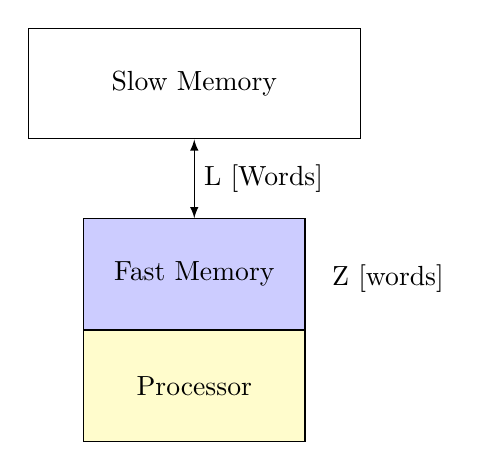
\begin{tikzpicture}[>=latex,rect/.style={draw=black, 
				rectangle, 
				fill=gray,
				fill opacity = 0.2,
				text opacity=1,
				minimum width=80pt, 
				minimum height = 40pt, 
				align=center}]
			\node[rect, fill=white,minimum width =120pt] (a1) {Slow Memory};
			\node[rect,below=1 of a1,fill=blue] (b1) {Fast Memory};
			\node[rect,label={[xshift=7em,yshift=1em]Z [words]},below=0 of b1,fill=yellow] (b2) {Processor};
			\draw[<->] (a1)--(b1)node[midway,right]{L [Words]};
		\end{tikzpicture}
	\end{wrapfigure}
	the basic model follows a modified von neumann model that consists of a slow but infinite \textbf{main memory} and smaller \textbf{fast memory}.
	There are \textbf{2 rules} associated with this model.
	
	\textbf{Local data rule:} Processor may only compute on data in fast memory.
	
	\textbf{Block transfer rule:} Slow-fast transfers in blocks of size \textbf{L} words.
	
	Because of these rules, transferring $x<L$ words from slow to fast memory will require a transfer of a full block of $L$ meaning $L-x$ unused words will be transferred. These blocks are likely at fixed place in slow memory, thus requiring us to think about \textbf{Block alignment}.
	
	This architecture also requires a different cost model. This model looks at the cost of \textbf{Work} just like normal, and also \textbf{Transfers}.
	
	\textbf{Work:} denoted $W(n)=$ number of computation operations.
	
	\textbf{Transfers:} denoted $Q(n;Z,L)=$ number of $L$-sized slow-fast transfers (loads and stores) this is also known as \textbf{I/O complexity}.
	\begin{mdframed}[style=Example]
		\textbf{Example:} Reduction of an array of size $n$.
		\vspace{2mm}
		
		$W(n) \geq n-1$ additions = $\Omega(n)$
		
		$Q(n;Z,L) \geq \lceil\frac{n}{L}\rceil$ transfers = $\Omega(\frac{n}{L})$
		\vspace{2mm}
		
		\noindent
		\textbf{Note:} Ceiling exists due to change of chunk misalignment.
	\end{mdframed}
	\begin{mdframed}[style=Quiz]
		\textbf{Quiz:} How many transfers are necessary in the worst case, assuming nothing about alignment?
		\vspace{2mm}
		
		\noindent
		\textbf{Answer:} $Q(n;Z,L) \leq \lceil n/L \rceil + 1$  If the array is not aligned then we'll need an extra transfer. Often ignore this detail if $N$ is massive.
	\end{mdframed}
	\begin{mdframed}[style=Quiz]
		\textbf{Quiz:} Give a simple (trivial) lower bound on the asymptotic number of transfers of an array of size $n$.
		\vspace{2mm}
		
		$W(n) = \Omega(n\log n)$ (comparison-based)
		
		$Q(n;Z,L) = \Omega(\lceil\frac{n}{L}\rceil)$
		\vspace{2mm}
		
		\noindent
		\textbf{Note:} Just the cost of reading the array. \textbf{$n$} because every word much be touched at least once. \textbf{$L$} in the best case read elements at one block at a time.  Ceiling makes this bound slightly tighter in the case that $L \nmid n$.
	\end{mdframed}
	%
	%Matrix Multiply quiz
	%
	\begin{mdframed}[style=Quiz]
		\textbf{Quiz:} Give a simple (trivial) lower bound on the asymptotic number of transfers of 2 matrices $C \leftarrow A \cdot B$ where $A, B, C$ are $nxn$ matrices.
		\vspace{2mm}
		
		$W(n) = \Omega(n^3)$ (non-strassen)
		
		$Q(n;Z,L) = \Omega(\frac{n^2}{L})$
		\vspace{2mm}
		
		\noindent
		\textbf{Note:} $n^2$ is just the number of elements, assuming we're able to load these into fast memory perfectly it will only take $n^2/L$ loads.
	\end{mdframed}
	%
	% Reduction Example algo%
	%
	\vspace{2mm}
	\subsection{I/O Reduction Example}
	How do we create algorithms with transfers in mind? How do we need to change the below algorithm?
	\begin{algorithm}
		\title{I/O Example: Reduction - Conventional}
		\begin{algorithmic}
			\State $s \gets 0$
			\For{$i \gets 0$ to $n-1$}
			\State $s \gets s + X[i]$
			\EndFor
		\end{algorithmic}
	\end{algorithm}
	\begin{algorithm}
		\title{I/O Example: Reduction - Local}
		\begin{algorithmic}
			\State Local $s \gets 0$
			\For{$i \gets 0$ to $n-1$ by $L$}
			\State Local $\hat{L} \gets$min$(n,i+L-1)$
			\State Local $y[0:\hat{L}-1] \gets X[i:(i+\hat{L}-1)]$
			\For{$di \gets 0$ to $\hat{L}-1$}
			\State $s \gets s + y[di]$
			\EndFor
			\EndFor
		\end{algorithmic}
	\end{algorithm}
	
	We'll need to pay attention to a few things, we'll need to make sure $s$ is already in memory using some term such as \textbf{local}, though this can be ignored usually. Most importantly for this algorithm we'll need to look at $X[i]$. Assuming X is aligned on an $L$-word boundary and that $n >> Z$.
	\begin{itemize}
		\item By $L$ exists to iterate at the block level, indicating that our steps are $L$ size.
		\item $\hat{L}$ step exists to determine if the block is of size L or a little bit smaller. (usually ignored detail).
		\item $y$ assignment is an explicit read (load) from slow memory to fast memory.
	\end{itemize}
	What is the Work and Transfers of this algorithm? $W(n) = \Theta(n)$ and $Q(n;Z,L)  = \Theta(\lceil\frac{n}{L}\rceil)$
	%
	% Quiz Matrix Vector Multiply
	%
	\begin{mdframed}[style=Quiz]
		\textbf{Quiz: } Matrix-vector Multiply $y \gets A \cdot x$
		
		\noindent
		\textbf{Assume}
		\begin{itemize}
			\item Rows are indexed by $i$ and columns by $j$
			\item A is column-major: $a_{ij} \leftrightarrow A[i + j \cdot n]$ (Records are stored where the next element follows in the column)
			\item $Z = 2n + O(L)$ (Fast memory can hold 2 vectors plus a little bit)
			\item $L | n$
			\item $x,y,A$ are aligned on $L$ (Ignore floors and ceilings)
		\end{itemize}
		
		\noindent
		\textbf{Given:} 2 algorithms, one (A) that iterates first through $i$ then $j$ vs an algorithm (B) which loops first through $j$ then $i$. These are identical in the RAM model.
		
		\noindent
		\textbf{Question:} In the I/O model which of the 2 algorithms performs fewer transfers?
		
		\noindent
		\textbf{Answer:} (B). Consider (A) because $j$ is the inner iteration, we'll need to look to the next row per inner loop leading to $Q(n;Z,L)  = \frac{3n}{L} + n^2$. $\frac{3n}{L}$ exists since we need to load each vector once at the start then write the final vector back. (B) on the other hand $Q(n;Z,L)  = \frac{3n}{L} + \frac{n^2}{L}$ since we get to load the elements in $L$ chunks.
	\end{mdframed}
	\subsection{Algorithmic Design Goals}
	\begin{enumerate}
		\item \textbf{Work Optimally: } Don't blow up the RAM model. If $W_*(n)$ is the RAM work then $W(n) = \Theta(W_*(n))$
		\item \textbf{High computation intensity: } Maximize intensity. Intensity can be defined as $I(n;Z,L) \equiv \frac{W(n)}{L \cdot Q(n;Z,L)}$. So the work divided by the number of words transferred. $Q(n;Z,L)$ being number of transfers and $L$ being the number of words per transfers. Also put $\frac{[ops]}{[Words]}$, measuring the data reuse of the algorithm. If this ratio is large it means we're doing more work per transfer. We do not want to optimize this at the expense of sub-optimal \textbf{work}.
	\end{enumerate}
	\subsection{Intensity, Balance, and Time}
	\begin{center}
		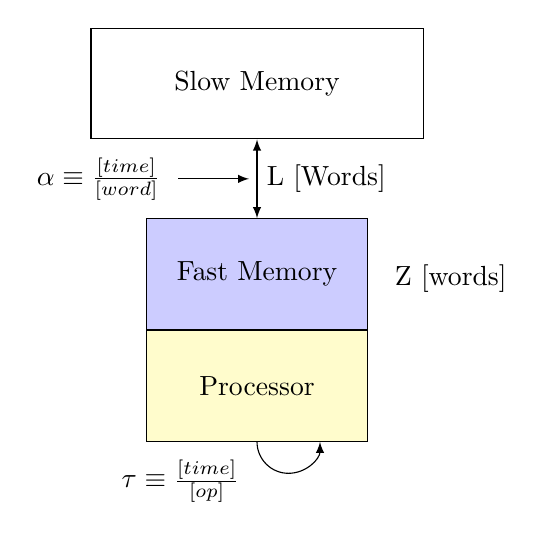
\begin{tikzpicture}[>=latex,rect/.style={draw=black, 
				rectangle, 
				fill=gray,
				fill opacity = 0.2,
				text opacity=1,
				minimum width=80pt, 
				minimum height = 40pt, 
				align=center}]
			\node[rect, fill=white,minimum width =120pt] (a1) {Slow Memory};
			\node[rect,below=1 of a1,fill=blue] (b1) {Fast Memory};
			\node[rect,label={[xshift=7em,yshift=1em]Z [words]},below=0 of b1,fill=yellow] (b2) {Processor};
			\draw[<->] (a1)--(b1)node[midway,right](bus){L [Words]};
			\draw[->] (b2.-90) arc (180:180+180:4mm)node[xshift=-.5cm,yshift=-.1cm,midway,below,left]{$\tau \equiv \frac{[time]}{[op]}$};
			\draw[->] ([xshift=-1cm]bus.west)--([xshift=-.1cm]bus.west)node[xshift=-1cm,left](alpha){$\alpha \equiv \frac{[time]}{[word]}$};
		\end{tikzpicture}
	\end{center}
	\begin{itemize}
		\item $T_{comp} = \tau W$ The time to complete just the \textbf{compute}.
		\item $T_{mem} = \alpha LQ$ The time to complete just the \textbf{transfers}.
	\end{itemize}
	Ideally the total time would be $T \geq$ max$(T_{comp},T_{mem})$ (assuming 100\% overlap). We can refactor this a bit into $\tau W \cdot$max$(1,\frac{\alpha/\tau}{w/(LQ)})$. $\tau W$ being the ideal computation time, with $(1,\frac{\alpha/\tau}{w/(LQ)})$ being the communication penalty, aka the price you pay for moving the data. We can simplify this equation further. Looking at $W/(LQ)$ is just the intensity, $[ops]/[word]$ thus $(1,\frac{\alpha/\tau}{I})$.
	
	The numerator is a factor known as ''machine balance`` $\equiv \alpha / \tau$ which also has a factor of $[ops]/[word]$ which means how many operations can be completed in the time it takes to move a word. $B \equiv \alpha / \tau \equiv $ ``machine balance'' meaning we can further simplify to $\tau W \cdot$max$(1,\frac{B}{I})$. The maximum time  $\tau W \cdot$max$(1 + \frac{B}{I})$. if there is no overlap you pay for computation and communication.
	
	\textbf{Normalized performance: } $R \equiv \frac{\tau W_*}{T} \leq \frac{W_*}{W} \cdot$min$(1,\frac{I}{B})$. The is inversely related to time, thus higher values are better.
	%
	% Quiz Intensity of Conventional Matrix Multiply
	%
	\begin{mdframed}[style=Quiz]
		\textbf{Quiz: } Intensity of Conventional Matrix Multiply. For a matrix $C \gets C + A \cdot B$ where we iterate through every row, every column then every element.
		
		\noindent
		\textbf{Assume:}
		\begin{itemize}
			\item $L = 1 word$ don't worry about alignment.
			\item $Z = 2n + O(1)$ Z is large enough to store 2 vectors plus some.
		\end{itemize}
		
		\noindent
		\textbf{Question:} What is the intensity of this algorithm?
		
		\noindent
		\textbf{Answer:} $I(n;z) = \theta(1)$. It is just constant. $W(n) = \Theta(n^3)$ and $Q(n;z) = \Theta(3n^2 + n^3)$.
	\end{mdframed}
	%
	% Block Matrix Multiply
	%
	\clearpage
	\begin{algorithm}
		\title{Block Matrix Multiply Algorithm}
		\begin{algorithmic}
			\For{$i \gets 0$ to $n-1$ by $b$}
			\For{$j \gets 0$ to $n-1$ by $b$}
			\State let $\hat{C} \equiv bxb$ block at $C[i,j]$b
			\For{$k \gets 0$ to $n-1$ by $b$}
			\State let $\hat{A} \equiv bxb$ block at $A[i,k]$
			\State let $\hat{B} \equiv bxb$ block at $B[k,j]$
			\State $\hat{C} \gets \hat{C} + \hat{A} \cdot \hat{B}$
			\EndFor
			\State $C[i,j]$block$\gets\hat{C}$
			\EndFor
			\EndFor
		\end{algorithmic}
	\end{algorithm}
	\begin{mdframed}[style=Quiz]
		\textbf{Quiz:} Given the Block Matrix Multiply Algorithm what is the intensity?
		
		\noindent
		\textbf{Assume:}
		\begin{itemize}
			\item $L = 1$
			\item $b | n$
			\item $n | Z$
			\item $Z=3b^2 + O(1)$
		\end{itemize}
		
		\noindent
		\textbf{Answer:} $I(n;Z) = \Theta(b$ or $\sqrt{Z})$. $\hat{C}$ requires $b^2$ to read the blocks and $\frac{n}{b} \cdot \frac{n}{b}$ times from the 2 loops. $n^2$ dominates meaning this is $n^2$ reads. The A and B loops are the same except for 3 loops meaning there are $\frac{n^3}{b}$ reads. Since Intensity is $W/(LQ)$ the answer is just $b$.
	\end{mdframed}
	%
	% Cache Quiz
	%
	\begin{mdframed}[style=Quiz]
		\textbf{Quiz: } Suppose you have an efficient machine for a matrix multiple at a particulay problem size. If the \textbf{machine balance} doubles, by how much should the size of fast memory increase?
		
		
		\noindent
		\textbf{Answer: } by \textbf{4}. Remember that  $R_{max} \equiv \frac{W_*}{W} \cdot$min$(1,\frac{I}{B})$. Since we know that $I$ of block matrix multiply is $\sqrt{Z}$ thus in order to compensate for $B$ increasing by 2, $Z$ needs to increase by 4.
	\end{mdframed}
	\clearpage
	\section{I/O Avoiding Algorithms}
	%
	% Io avoiding algos
	%
	\begin{mdframed}[style=Quiz]
		\textbf{Given:}
		\begin{itemize}
			\item Volume of data to sort $\equiv r \cdot n = 1 PiB (=2^{50})$ Bytes
			\item Record (item) size $\equiv r = 256$ Bytes
			\item Fast memory size $\equiv r \cdot z = 64 GiB (=2^{36}B)$
			\item Memory transfer size $\equiv r \cdot L = 32 KiB (=2^{15}B)$
		\end{itemize}
		
		\noindent
		\textbf{Question:} What is the performance of various equations?
		
		\noindent
		\textbf{Answer:}
		\begin{center}
			
			\begin{tabular}{cccccc}
				$n\log_2n$ & $n\log_2\frac{n}{L}$ & $n$ & $\frac{n}{L}\log_2\frac{n}{L}$ &$\frac{n}{L}\log_2\frac{n}{Z}$ &$\frac{n}{L}\log_{\frac{Z}{L}}\frac{n}{Z}$\\
				\hline
				185& 154& 4.40& 1.20 &0.275& 0.0523 \\
			\end{tabular}
		\end{center}
		
		\noindent
		\textbf{Note:} importantly the biggest improvement comes when going from $n\log_2$ to $\frac{n}{L}\log_2$ because we we iterate through the data, we do it in $L$ chunks vs one at a time. The other big improvement comes from going from $\log_2$ to $\log_{\frac{Z}{L}}$ This improvement involves the capacity of fast memory $Z$, this maximises useage of fast memory.
	\end{mdframed}
	\subsection{External Memory Mergesort} Imagine an array with n elements. How can we perform a merge sort on that algorithm? First we divide the array into blocks of $Z$ size.
	\begin{center}
		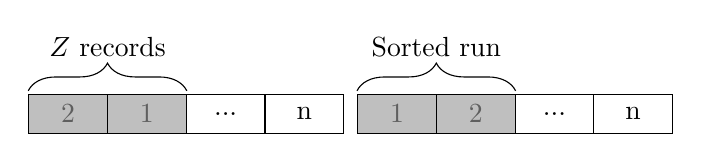
\begin{tikzpicture}
			\node[rectangle,
			draw,
			text = black
			, fill=gray
			,fill opacity=.5
			,minimum width = 1cm
			, minimum height =.5cm] (1) at (0,0) {2};
			\node[rectangle,
			draw,
			text = black
			, fill=gray
			,fill opacity=.5
			,minimum width = 1cm
			, minimum height =.5cm] (2) [right of=1] {1};
			\node[rectangle,
			draw,
			text = black
			,minimum width = 1cm
			, minimum height =.5cm] (...) [right of=2] {...};
			\node[rectangle,
			draw,
			text = black
			,minimum width = 1cm
			, minimum height =.5cm] (n) [right of=...] {n};
			\draw [decorate,
			decoration = {brace,raise=1pt,amplitude=10}] (1.north west) -- (2.north east)node[pos=0.5,above=10pt,black]{$Z$ records};
					\node[rectangle,
			draw,
			text = black
			, fill=gray
			,fill opacity=.5
			,minimum width = 1cm
			, minimum height =.5cm] (3) [xshift=5,right of=n] {1};
			\node[rectangle,
			draw,
			text = black
			, fill=gray
			,fill opacity=.5
			,minimum width = 1cm
			, minimum height =.5cm] (4) [right of=3] {2};
			\node[rectangle,
			draw,
			text = black
			,minimum width = 1cm
			, minimum height =.5cm] (...2) [right of=4] {...};
			\node[rectangle,
			draw,
			text = black
			,minimum width = 1cm
			, minimum height =.5cm] (n2) [right of=...2] {n};
			\draw [decorate,
			decoration = {brace,raise=1pt,amplitude=10}] (3.north west) -- (4.north east)node[pos=0.5,above=10pt,black]{Sorted run};
		\end{tikzpicture}
	\end{center}
We then load this chunk and sort it writing it back to the array producing a \textbf{(sorted) run}. repeat this process until all $\frac{n}{fZ}$ chunks are sorted runs. This is \textbf{Phase 1} of the procedure.
\begin{mdframed}[style=Quiz]
	\textbf{Question:} What are the total Asymptotic costs?
	
	\noindent
	\textbf{Answer:}
	\begin{enumerate}
		\item Read Chunk $o(\frac{n}{L})$
		\item comparisons $o(n\log z)$
		\item Read Chunk $o(\frac{n}{L})$
	\end{enumerate}
\end{mdframed}

	\clearpage
	\section{Algorithmic Time - Energy and Power}
	%
	%ALGORITHMIC TIME%
	%
	\subsection{Balance Principles}
	\begin{equation} \label{work}
		work W=W(n) = total ops
	\end{equation}
	the equation \ref{work} states some shit
	
	
	Span $D=D(n)$ [ops]
	
	Transactions $Q=Q(n;Z,L)<=w$
	
\end{document}
